\documentclass{homework}
% \usepackage{graphicx} % Required for inserting images
\usepackage{amsmath}
\usepackage{gensymb}
\usepackage{subfig}
\usepackage{float}
% \usepackage{algorithm}
\usepackage{algorithm}
\usepackage{algpseudocode}

\class{APPM 5560}
\title{Homework 2}
\author{Sean Jennings}
\date{January 31, 2024}

\definecolor{dkgreen}{rgb}{0,0.6,0}
\definecolor{gray}{rgb}{0.5,0.5,0.5}
\definecolor{mauve}{rgb}{0.58,0,0.82}

\lstset{frame=tb,
  language=Python,
  aboveskip=3mm,
  belowskip=3mm,
  showstringspaces=false,
  columns=flexible,
  basicstyle={\small\ttfamily},
  numbers=none,
  numberstyle=\tiny\color{gray},
  keywordstyle=\color{blue},
  commentstyle=\color{dkgreen},
  stringstyle=\color{mauve},
  breaklines=true,
  breakatwhitespace=true,
  tabsize=3
}


\begin{document}
\maketitle

\section{Problem 1}
The MGF of the binomial $X \sim \text{Binomial}(n, p)$ is given by:
\begin{equation*}
    \sigma_X{s} = (pe^s + 1 - p)^n
\end{equation*}
Since the MGF of the sum of independent random variables is the product of
the individual MGFs, we have:
\begin{align*}
    \sigma_{X+Y}(s) = \sigma_X(s) \sigma_Y(s) \\
        &= (pe^s + 1 - p)^n (pe^s + 1 - p)^m \\
        &= (pe^s + 1 - p)^{n + m}
\end{align*}
It follows that $X+Y \sim \text{binomial}(n+m, p)$, because two R.V. are identical
iff their MGFs are equal.

This makes sense because a binomial is the number of independent Bernoulli trials
which end in success. So the sum of two independent binomials with the same
parameter $p$ is just the sum $n+m$ independent Bernoulli trials,
which is equavalent to a binomial with parameters $n+m$ and $p$.

\section{Problem 2}

We differentiate both sides of the expression
\begin{equation}
    {\bf E}[X^n] = A_n \sigma^n = \int_{-\infty}^{\infty}
        \frac{1}{\sqrt{2\pi}\sigma} x^n e^{\frac{-x^2}{2\sigma^2}} dx
    \label{eq:expectation-n}
\end{equation}
by $\sigma$ to obtain an expression for ${\bf E}[X^n]$. First,
\begin{equation}
    \frac{d}{d\sigma}\biggl(A_n \sigma^n\biggr) = nA_n \sigma^{n-1}.
    \label{eq:derivative-lhs}
\end{equation}
We will write the function $E: \R \to \R$ as defined by
\begin{equation*}
    E(\sigma) = e^{\frac{-z^2}{2\sigma^2}}
\end{equation*}
for brevity. Taking the derivative of $E$ yields:
\begin{equation*}
    \frac{dE}{d\sigma} = \frac{x^2}{\sigma^3} E(\sigma)
\end{equation*}
Thus, the derivative of the right-hand side of equation \ref{eq:expectation-n}
reduces as follows:
\begin{align*}
    \frac{d}{d\sigma}\biggl(
        \int_{-\infty}^{\infty}
                \frac{1}{\sqrt{2\pi}\sigma} x^n E(\sigma) dz
    \biggr) &= \frac{1}{\sqrt{2\pi}} \frac{x^n}{\sigma} \biggl(
        \frac{x^2}{\sigma^3} E(\sigma)
    \biggr)
        - \frac{x^n}{\sigma^2} E(\sigma) dz \\
        &= \frac{1}{\sigma^3}
        \int_{-\infty}^{\infty} \frac{1}{\sqrt{2\pi}\sigma} x^{n+2} E(\sigma) dx
        - \frac{1}{\sigma}
        \int_{-\infty}^{\infty} \frac{1}{\sqrt{2\pi}\sigma} x^{n} E(\sigma) dx \\
        &= \frac{1}{\sigma^3} {\bf E}[X^{n+2}] - \frac{1}{\sigma} {\bf E}[X^n].
\end{align*}
Equating this result to equation \ref{eq:derivative-lhs} and substituing
${\bf E}[X^n] = A_n \sigma^n$ yields
\begin{equation*}
    nA_n \sigma^{n-1} = \frac{1}{\sigma^3} A_{n+2}\sigma^{n+2} - \frac{1}{\sigma} A_n \sigma^n.
\end{equation*}
Dividing by $\sigma^{n-1}$ eliminates the dependence upon $\sigma$:
\begin{equation*}
    nA_n = A^{n+2} - A_n
\end{equation*}
which simplifies to the recursive relation
\begin{equation*}
    A_{n+2} = (n+1) A_n
\end{equation*}
for even $n\geq 2$. We differentiate the MGF to find the initial $A_2$ which
starts the recursion.
\begin{align*}
    \sigma_X(s) &= e^{1/2 \sigma^2 s^2} \\
    \sigma_X'(s) &= \sigma^2 s e^{1/2 \sigma^2 s^2} \\
    \sigma_X''(s) &= \biggl(
        \sigma^4 s^2 + \sigma^2
    \biggr) e^{1/2 \sigma^2 s^2}.
\end{align*}

Taking the second derivative with $s=0$, we have
\begin{equation*}
    {\bf E}[X^2] = \sigma_X''(0) = \sigma^2  
\end{equation*}
and thus $A_2=1$, completing our expression for ${\bf E}[X^n]$.

Additionally, a recursive expression for ${\bf E}[X^n]$ can be derived from
the MGF as follows. First, the $n$th derivative of the MGF can be written
\begin{equation}
    \sigma_X^{(n)} = p_n(s) e^{1/2 \sigma^2 s^2}
    \label{eq:mgf-poly}
\end{equation}
where $p_n(s)$ is an $n$th order polynomial which can be defined
recusively
\begin{equation*}
    p_{n+1}(s) = \sigma^2 s p_n(s) + p_n'(s)
\end{equation*}
and $p_n'(s)$ is the derivative of the $n$th polynomial. The initial
$p_0$ is given by $p_0(s) = 1$.

This recursive relationship can easily be seen by applying the chain
rule to differentiate equation \ref{eq:mgf-poly}.

If we write the polynomial $p_n(s)$ as
\begin{equation*}
    p_n(s) = a_{n,0} + a_{n,1} s + \cdots + a_{n,n} s^n
\end{equation*}
where $a_{n,i}\in\R$ for all $i=[0,\dots,n]$, then the expected value 
${\bf E}[X^n]$ is given by the constant coefficient of $p_n$:
\begin{equation*}
    {\bf E}[X^n] = \sigma_X^{(n)}(0) = p_n(0) = a_{n,0}
\end{equation*}


\section{Problem 3}
Algorithm \ref{alg:discrete-rv} describes an efficient algorithm to generate a
generate discrete random variable $X$. It follows the inverse tranform method,
and also uses a permutation to improve
efficiency by checking the most probable outcomes first.

Implementation details (such as verifying that the probability mass function (PMF)
is normalized) are omitted for clarity.

\begin{algorithm}
    \caption{Discrete Random Variable}\label{alg:discrete-rv}
\begin{algorithmic}
    \Function{DiscreteRV}{p, X}
               \Comment Generate discrete random variable, given arrays
        \State \Comment of values, $X$, each with associated probability, $p$.

        \State $n \gets $ length(p)
        \State $\sigma \gets $reverse(argsort($p$))
        \Comment Save the indexes which give $p$ in descending order

        \State $u  \sim  $Uniform$(0, 1)$
        \State $total \gets 0$
        \For {$i \gets 1$ {\bf  to }n}
            \State $total \gets total + p[\sigma(i)]$
            \If {$total \geq u$}
                \State \Return $X[\sigma(i)]$
            \EndIf \Comment Else: continue looping
        \EndFor
    \EndFunction
\end{algorithmic}
\end{algorithm}

Algorithm \ref{alg:specific-drv} details the function call to simulate
the specific random variable in question:
\begin{algorithm}
    \caption{Sample specific Random Variable}\label{alg:specific-drv}
\begin{algorithmic}
    \State $p \gets [0.01, 0.05, 0.9, 0.04]$
    \State $X \gets [1, 2, 3, 4]$
    \State \Return DiscreteRV(p, X)
\end{algorithmic}
\end{algorithm}

\section{Problem 4}
The following pseudocode simulates the distribution of interest via the
acceptance-rejection method. We sample from the distribution
$U,X \sim $Uniform$(0, 1)$ and accept when
\begin{equation*}
    cU \leq f(X)
\end{equation*}
where $C>0$ is given by
\begin{equation*}
    C = \max_{0\leq x \leq 1} f(x) = 1.5.
\end{equation*}
The pseudocode is given in Algorithm \ref{alg:accept-reject}

\begin{algorithm}
    \caption{Simulating via Acceptance-Rejection Method}\label{alg:accept-reject}
\begin{algorithmic}
    \Loop
        \State $u  \sim  $Uniform$(0, 1)$
        \State $x  \sim  $Uniform$(0, 1)$
        \If {$4x(1-x) \geq u$}
            \State \Return x
        \EndIf
    \EndLoop
\end{algorithmic}
\end{algorithm}

\section{Problem 5}
We sample two exponential variables $X$ and $Y$ via the inverse transform method
and then divide samples of $Y$ by $X$ to generate $Z$. In figure
\ref{fig:z-simulation}, we see
that the histogram sampled points aligns closely with the analytic solution for
the PDF of $Z$, found in HW1 to be
\begin{equation*}
    f_Z(z) = \biggl\{
        \begin{array}{ll}
            \frac{\lambda_1 \lambda_2}{(\lambda_1 + \lambda_2 z)^2}
                &\quad \text{if } z>=0 \\
            0 &\quad \text{otherwise.}
        \end{array}
    \biggr.
\end{equation*}

\begin{center}
    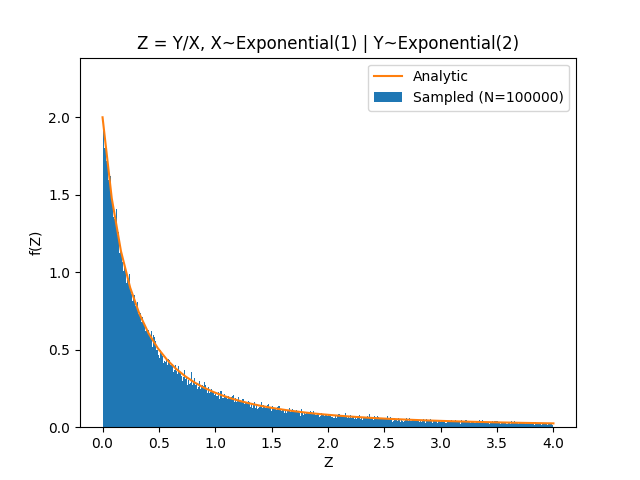
\includegraphics[width=0.8\linewidth]{Images/problem5.png}
    \captionof*{figure}{Problem 5: Simulation of random variable Z}
    \label{fig:z-simulation}
\end{center}

The plot is truncated at $z=4$, but we note that approximately 11\% of samples
have $z>4$. The code which generates that plot in Python is shown in
Listing \ref{lst:prob5} below:
\begin{lstlisting}[caption=Problem 5 Python Code, label=lst:prob5]

from numpy import log, linspace
from numpy.random import uniform
import matplotlib.pyplot as plt

def exponential(lambda_, n):
    # Generate (n,) array of uniform RVs.
    u = uniform(0, 1, n)
    # Compute exponential via inverse transform method.
    return -1/lambda_ * log(u)

def problem5():
    N = 100_000
    lambda_1 = 1
    lambda_2 = 2
    max_z = 4
    # Sample X, Y from exponential distrution (with N datapoints) and 
    # perform element-wise division to compute Z.
    x = exponential(lambda_1, N)
    y = exponential(lambda_2, N)
    z = y / x
    # Compute analytically determined PDF.
    z_pdf = linspace(0, max_z)
    f_z = lambda_1 * lambda_2/ (lambda_1 + lambda_2 * z_pdf)**2

    fig = plt.figure()
    histogram(z, range=(0, max_z), density=True, bins=500)
    plt.plot(z_pdf, f_z)

    plt.xlabel("Z")
    plt.ylabel("f(Z)")
    plt.title("Z = Y/X, X~Exponential(1) | Y~Exponential(2)")
    plt.legend(["Analytic", f"Sampled (N={N})"])

    fig.savefig("Images/problem5.png")

    plt.show()
\end{lstlisting}

\section{Problem 6}
First we compute the CDF of $X$:
\begin{align*}
    F_X(x) &= \int_{-\infty}^{x} f(y) dy \\
        &= \biggl\{
            \begin{array}{ll}
                \int_{1}^{x} 3y^{-4} dy &\quad \text{if }x>1 \\
                0 &\quad \text{otherwise}
            \end{array}
        \biggr. \\
        &= \biggl\{
            \begin{array}{ll}
                -y^{-3} \eval_1^x  &\quad \text{if }x>1 \\
                0 &\quad \text{otherwise}
            \end{array}
        \biggr. \\
        &= \biggl\{
            \begin{array}{ll}
                1 - x^{-3}  &\quad \text{if }x>1 \\
                0 &\quad \text{otherwise}
            \end{array}
        \biggr.
\end{align*}

From this we compute the inverse transform from $U = F(X)$ with $U \sim $Uniform$(0, 1)$
and find
\begin{align*}
    U = F(X) &= 1 - x^{-3} \\
        X^{-3} &= 1 - U = W \\
        X &= W^{-1/3}
\end{align*}
where for efficiency, we have substituted $W \sim $Uniform(0,1) for $1-U$ since their
distributions are identical.

We compute the theoretical mean from the PDF to be
\begin{align*}
    {\bf E}[X] &= \int_1^\infty xf(x) dx \\
        &= \int_{1}^{\infty} 3x^{-3} \\
        &= \frac{3}{2}x^{-2} \eval_1^\infty \\
        &= \frac{3}{2}.
\end{align*}
We compute a mean of about 1.5014 numerically, which signals no obvious error
in our implementation. The histogram shown in figure \ref{fig:power-law-simulation}
also shows the sampled variable coincides closely with the PDF.
\begin{center}
    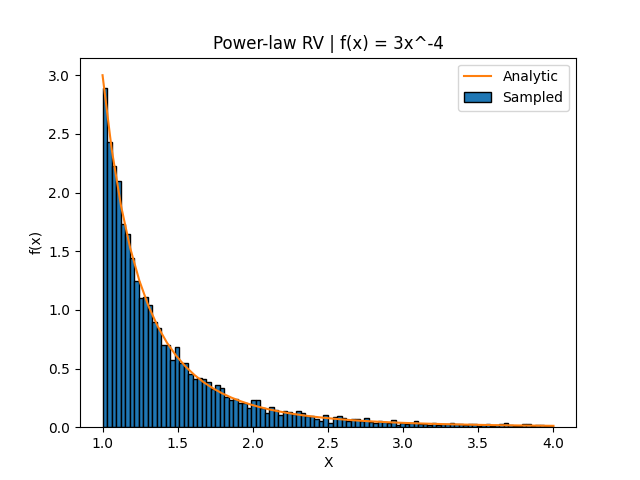
\includegraphics[width=0.8\linewidth]{Images/problem6.png}
    \captionof*{figure}{Problem 6: Simulation of Power Law distribution}
    \label{fig:power-law-simulation}
\end{center}
The code is found in Listing \ref{lst:prob6}

\begin{lstlisting}[caption=Problem 6 Code, label=lst:prob6]

from numpy import log, linspace
from numpy.random import uniform
import matplotlib.pyplot as plt

def problem6():
    N = 10_000
    x_max = 4
    # Sample Uniform distribution with N data points
    u = uniform(0, 1, N)
    # Simulate X using inverse tranform method.
    x = 1 / u ** (1/3)
    # Compute PDF over range
    x_range = np.linspace(1, x_max)
    f_x = 3 / x_range**4

    # Plot histogram of sampled points alongside PDF.
    fig = plt.figure()
    histogram(x, density=True, range=(1, x_max), bins=100, edgecolor='black')
    plt.plot(x_range, f_x)

    plt.title("Power-law RV | f(x) = 3x^-4")
    plt.xlabel("X")
    plt.ylabel("f(x)")
    plt.legend(["Analytic", "Sampled"])
    
    # Display results
    print(f"Mean: {np.mean(x)}")
    fig.savefig("Images/problem6.png")

    plt.show()
\end{lstlisting}

\section{Problem 7}

We will compute $Y$ via the inverse transform method. We compute $Y = F^{-1}(U)$
as follows:
\begin{align*}
    U = F(Y) &= \frac{e^y}{1 + e^y} \\
    &\Rightarrow \frac{1 + e^y}{e^y} = e^{-y} + 1 = \frac{1}{U} \\
    &\Rightarrow Y = -\ln \biggl(\frac{1}{U} - 1\biggr) = \ln\biggl(\frac{U}{1-U}\biggr)
\end{align*}
After computing $Y$, we can perform a second step of the inverse transform
method to simulate $X$, as summarized in Algorithm \ref{alg:exponential-y2}.
We omit pseudocode for the exponential as the Python implementation can be seen
in Listing \ref{lst:prob5}.

\begin{algorithm}
    \caption{Exponential with $\lambda=Y^2$}\label{alg:exponential-y2}
\begin{algorithmic}
    \State $u \sim$ Uniform(0, 1)
    \State $y \gets \ln(\frac{u}{1-u})$
    \State \Return Exponential($Y^2$)
\end{algorithmic}
\end{algorithm}

\section{Problem 8}
As alluded to in Problem 1, we can simultate a binomial R.V. either
by
\begin{enumerate}
    \item simulating $X_i \sim $Bernoulli$(p)$ for $i$ from 1 to $n$ and taking
        the sum $X = \sum_{i=1}^n X_i$, or
    \item using the inverse transform method for discrete random variables,
        where $p_X(k)$ for each $k\in[0,\dots,n]$ is computed from the closed
        form of the binomial PMF.
\end{enumerate}

Pseudocode is provided in Algorithms \ref{alg:bi-via-bern} and \ref{alg:bi-inv-trans},
respectively. Note: Algorithm \ref{alg:bi-inv-trans} makes use of the "DiscreteRV" function
described in Algorithm \ref{alg:discrete-rv}.

\begin{algorithm}
    \caption{Generate Binomial($n,p$) via Bernoulli trials}\label{alg:bi-via-bern}
\begin{algorithmic}
    \State $X \gets 0$
    \For {$i \gets 1$ {\bf  to }$n$}
        \State $u \sim$ Uniform(0, 1)
        \If{$u < p$}
            \State $X \gets X + 1$
        \EndIf
    \EndFor
    \State \Return X
\end{algorithmic}
\end{algorithm}

\begin{algorithm}
    \caption{Generate Binomial($n,p$) via Inverse transform}\label{alg:bi-inv-trans}
\begin{algorithmic}
    \State $X \gets [0,\dots,n]$
    \State $p \gets \biggl[
        \binom{n}{k} p^k (1-p)^{n-k}
    \biggr] \forall k\in X$
    \State \Return DiscreteRV(p, X)
\end{algorithmic}
\end{algorithm}

\section{Problem 9}
\begin{letterenum}
\item Intuitively, dish 2 should be eaten most in the long-run since the probability
of transitioning from both dish 1 and 3 on the previous day are $>0.5$, and there is also
a high probability (0.7) of remaining on dish 2 for consecutive days in a row.

\item The probability of eaching dish $i$ on day $t+1$ is given by the total probability
law:
\begin{align*}
    P^{t+1}(i) &= \sum_{j=1}^{3} {\bf P}(\text{transition } j \to i |
                                   \text{ eats dish }j \text{ on day }t)
                            {\bf P}(\text{eats dish }j \text{ on day }t) \\
        &= \sum_{j=1}^{3}{\bf P}(\text{transition } j \to i |
                                   \text{ eats dish }j \text{ on day }t)
            P^t(j).
\end{align*}
Enumerating these summations yields expressions for each $i\in\{1, 2, 3\}$:
\begin{equation*}
    \begin{array}{llll}
        P^{t+1}(1) &=            &\quad 0.1 P^t(2) &+ 0.2 P^t(3) \\
        P^{t+1}(2) &= 0.5 P^t(1) &+ 0.7 P^t(2) &+ 0.8 P^t(3) \\
        P^{t+1}(3) &= 0.5 P^t(1) &+ 0.2 P^t(2)
    \end{array}
\end{equation*}

\item The previous system of equations can be written as a linear transformation
${\bf P}(t+1) = M{\bf P}(t)$ with matrix $M$ given by
\begin{equation*}
    M = \mat{
        0 & 0.1 & 0.2 \\
        0.5 & 0.7 & 0.8 \\
        0.5 & 0.2 & 0
    }.
\end{equation*}

\end{letterenum}






\end{document}
